\documentclass[13pt, t]{beamer}

% Presento style file
\usepackage{config/presento}
\usepackage{ulem}

% custom command and packages
% custom packages
\usepackage{textpos}
\setlength{\TPHorizModule}{1cm}
\setlength{\TPVertModule}{1cm}

\newcommand\crule[1][black]{\textcolor{#1}{\rule{2cm}{2cm}}}



% Information
\title{\huge Современные цифровые методы и технологии консервации}
\author[shortname]{Г. Мороз }
\date{\begin{center} 
\large 20 апреля 2018 г.
\end{center}}

\begin{document}

\begin{frame}[plain]
\maketitle
\end{frame}

\framecard[colorblue]{{\color{colorwhite} \huge цифровые методы и базы данных для объектов культуры}}

\begin{frame}{Мы уже обсуждали некоторые базы данных…}
\begin{itemize}
\item \href{https://www.gutenberg.org/}{\alert{Проект Гутенберг: https://www.gutenberg.org/}}
\item \href{https://www.europeana.eu}{\alert{Europeana Collections: https://www.europeana.eu}}
\item \href{https://dp.la/}{\alert{Digital Public Library of America: https://dp.la/}}
\item \href{https://www.hathitrust.org/}{\alert{HathiTrust digital library: https://www.hathitrust.org/}}
\item \href{https://www.rsl.ru/}{\alert{Российская Государственная Библиотека: https://www.rsl.ru/}}
\end{itemize}
\end{frame}

\begin{frame}{Диджитализацию/интерактивизацию музеев мы тоже обсуждали…}
\begin{itemize}
\item экспонаты переезжают в интернет, например, \href{https://www.museum-digital.de}{https://www.museum-digital.de}
\item музей переезжает в интернет, например, \href{http://www.louvre.fr/en/visites-en-ligne\#tabs}{Лувр}, \href{http://www.britishmuseum.org/with_google.aspx}{Британский музей}, \href{http://www.nga.gov/exhibitions/webtours.htm}{Национальная галерея искусства в Вашингтоне}
\item экспозиции дополняются при помощи технологий
\begin{itemize}
\item аудиогид
\item QR-коды
\item очки дополненной реальности
\item \href{https://www.youtube.com/watch?time_continue=154&v=XYRjaZl08lQ}{мультитач-экран}, \href{https://www.youtube.com/watch?v=qWJqd6lyJ-E}{еще пример}
\item \href{https://www.youtube.com/watch?v=BmadTQNrAeA}{интерактивные книжки}
\end{itemize}
\vfill 
Можно пытаться объединить самую разнородную информацию в одну антологию:
\item \href{https://www.youtube.com/watch?time_continue=133&v=uQQGgYPRWfs}{A virtual time machine for Venice}
\end{itemize}
\end{frame}

\framecard[colorblue]{{\color{colorwhite} \huge цифровые методы и реставрация}}

\begin{frame}{Mosaic floors in the North-West Church of Sussita}
\begin{center}
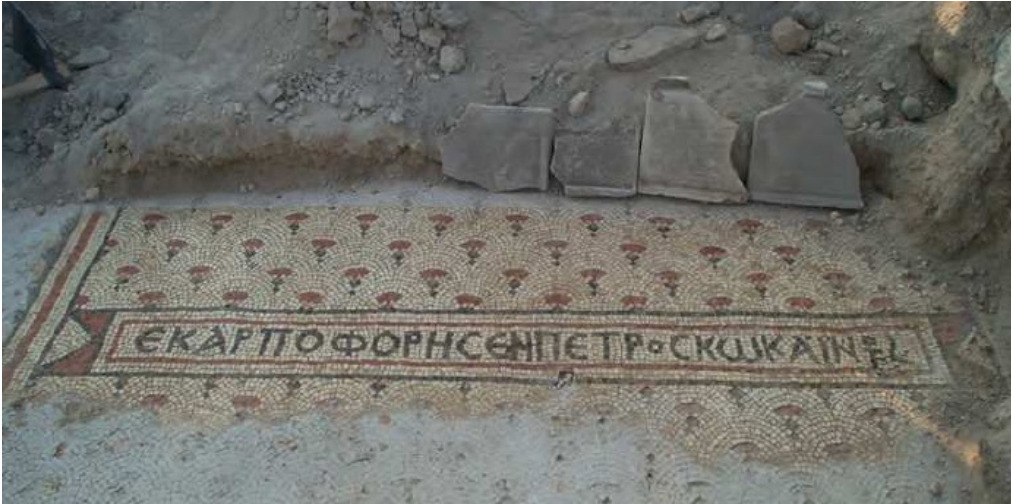
\includegraphics[width=0.6\linewidth]{images/01-Mosaik.jpg}
\pause
\vfill
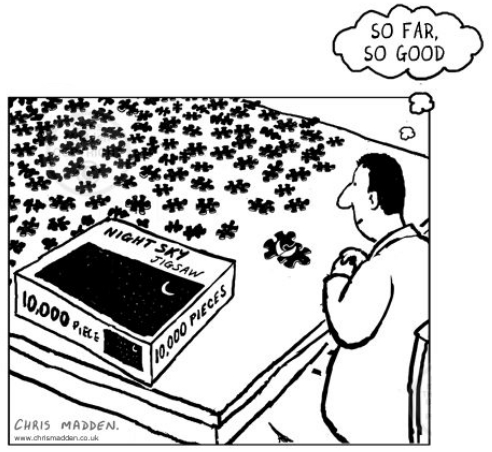
\includegraphics[width=0.5\linewidth]{images/02-Mosaik.jpg}
\end{center}
\end{frame}

\begin{frame}{Мозаики и фрески}
\begin{itemize}
\item создаем базу данных фрагментов
\item автоматически пытаемся оценить вероятность стыков на основании цвета, типа мазка, разных геометрических параметров и т. п.
\pause
\item а дальше эксперт проверяет на стыковку в разы меньше пар фрагментов
\end{itemize}
\end{frame}

\framepic{images/03-original.jpg}{\medskip \color{colorwhite} \Large  оригинальное {\small \hfill из [Shacham, Haik, Yitzhaky 2007]}}
\framepic{images/04-degraded.jpg}{\medskip \color{colorwhite} \medskip \Large  искаженное   {\small \hfill  из [Shacham, Haik, Yitzhaky 2007]}}
\framepic{images/05-restored.jpg}{\medskip \color{colorwhite} \smallskip \Large  восстановленное {\small \hfill из [Shacham, Haik, Yitzhaky 2007]}}

\begin{frame}{Реставрации и цифровая обработка изображения?}
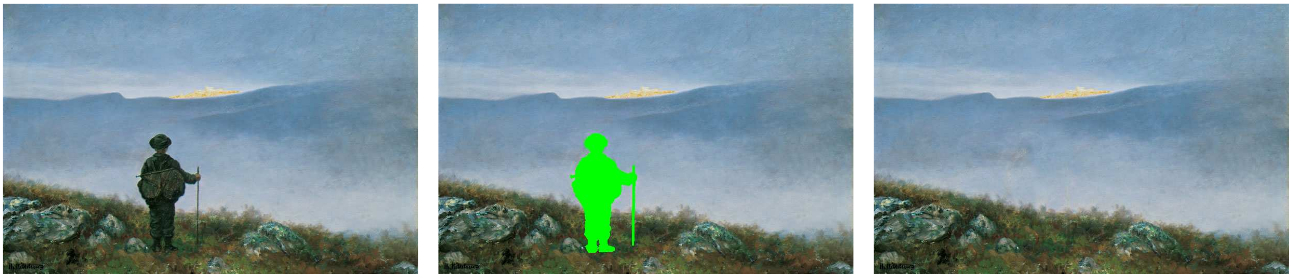
\includegraphics[width=\linewidth]{images/06-Kittelsen.jpg}\\

`Soria Moria' painting by Theodor Kittelsen.
\vfill
Oncu Feier, Alexandra Ioana. Digital Inpainting for Artwork Restoration: Algorithms and Evaluation, 2012
\end{frame}

\begin{frame}{Реставрации и цифровая обработка изображения?}
\begin{itemize}
\item Обработка изображения может помочь ручной реставрации
\begin{itemize}
\item можно попробовать разные способы
\item можно наложить черновики
\item можно воссоздать трюки, использовавшиеся художниками (например, эффект камеры-обскура или других линз)
\end{itemize}
\item Более быстрое и дешевое получение изображения
\begin{itemize}
\item для аудитории музеев
\item для получения финансовой поддержки
\end{itemize}
\end{itemize}
\end{frame}

\begin{frame}{Реставрации и цифровая обработка изображения?}
Но как измерить качество реставрации?\\
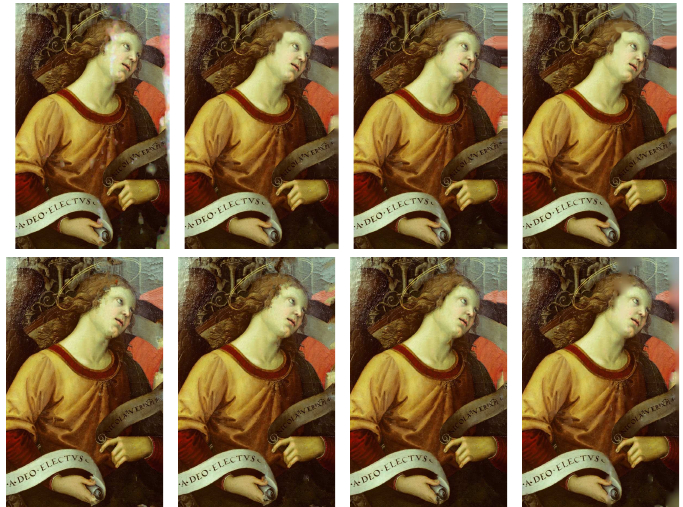
\includegraphics[width=0.95\linewidth]{images/07-Angel.jpg}
\end{frame}

\begin{frame}{Реставрации и цифровая обработка изображения?}
Но как измерить качество реставрации?\\
\begin{itemize}
\item мнение экспертов
\item мнение наивных зрителей
\item метрики качества изображения (PSNR, MSE, spatial-CIELAB, SSIM, ASVS, DN)
\end{itemize}
\end{frame}

\framepic{images/08-3d.jpg}{3D-модели керамических экспонатов (National Museum Cardiff) \\ {~} {\small \hfill из [Younan 2014]}}

\begin{frame}{Реставрации и 3D-моделирование?}
\begin{itemize}
\item Обработка изображения может помочь ручной реставрации
\begin{itemize}
\item можно попробовать разные способы
\item можно наложить черновики
\item можно воссоздать трюки, использовавшиеся артистами
\end{itemize}
\item Более быстрое и дешевое получение изображения
\begin{itemize}
\item для аудитории музеев
\item для получения финансовой поддержки
\end{itemize}
\end{itemize}
\end{frame}

\begin{frame}{Будущее...}
А что если мы создадим единую базу данных содержащую цифровые копии известных произведений искусства/культуры...
\end{frame}

\framecard[colorblue]{{\color{colorwhite} \huge Спасибо за внимание! \bigskip\\
\Large Пишите письма\\
agricolamz@gmail.com}}

\end{document}